\documentclass[onecolumn, draftclsnofoot,10pt, compsoc, tikz]{IEEEtran}
\usepackage{graphicx}
\usepackage{url}
\usepackage{setspace}
\usepackage{array}
\usepackage{pgfgantt}
\usepackage{color}
\usepackage{listings}

\usepackage{geometry}
\geometry{textheight=9.5in, textwidth=7in}

\def \CapstoneTeamName{		Ecological Footprint Team}
\def \CapstoneTeamNumber{		77}
\def \GroupMemberOne{			Rohan Barve}
\def \GroupMemberTwo{			Sathya Ramanathan}
\def \GroupMemberThree{			Dominic Wasko}
\def \CapstoneProjectName{		Ecological Footprint App}
\def \CapstoneSponsorCompany{	Oregon State University Sustainability}
\def \CapstoneSponsorPerson{		Brandon Trelstad} % change to brandon

\def \DocType{Winter Progress Report}
			
\newcommand{\NameSigPair}[1]{\par
\makebox[2.75in][r]{#1} \hfil 	\makebox[3.25in]{\makebox[2.25in]{\hrulefill} \hfill		\makebox[.75in]{\hrulefill}}
\par\vspace{-12pt} \textit{\tiny\noindent
\makebox[2.75in]{} \hfil		\makebox[3.25in]{\makebox[2.25in][r]{Signature} \hfill	\makebox[.75in][r]{Date}}}}
\renewcommand{\NameSigPair}[1]{#1}


\begin{document}
\begin{titlepage}
    \pagenumbering{gobble}
    \begin{singlespace}
        \hfill 
        \par\vspace{.2in}
        \centering
        \scshape{
	 \huge \DocType \par
            \huge CS 462 Capstone - Winter Term \par
            {\large\today}\par
            \vspace{.5in}
            \textbf{\Huge\CapstoneProjectName}\par
            \vfill
            {\large Prepared for}\par
            \Huge \CapstoneSponsorCompany\par
            \vspace{5pt}
            {\Large\NameSigPair{\CapstoneSponsorPerson}\par}
            {\large Prepared by }\par
            Group\CapstoneTeamNumber\par
            \CapstoneTeamName\par 
            \vspace{5pt}
            {\Large
                \NameSigPair{\GroupMemberOne}\par
                \NameSigPair{\GroupMemberTwo}\par
                \NameSigPair{\GroupMemberThree}\par
            }
            \vspace{20pt}
        }
        
        \begin{abstract}
        	For our Senior Capstone project, we decided to work with the sustainability department here at Oregon State University to create a greener solution for the community. 
	We have agreed with our client on the basis of creating an ecological footprint calculator specifically for the city of Corvallis.
	An ecological footprint is essentially a measurement of land area that is required to sustain a given population. 
	Through this calculator, we can measure individually how much each person consumes the overall available land/water resources. 
	We will be talking about the ecological problems we face today, the proposed solution, and our projects scope.

        \end{abstract}  
        
        
    \end{singlespace}
\end{titlepage}
\newpage
\pagenumbering{arabic}
\tableofcontents
\listoffigures
\clearpage

\section{Project Purpose \& Goals}
The purpose of this project is to create a mobile application for Android smart phones that will allow users to measure an approximation of their ecological footprint. 
The goals of this project are to provide users with a means to calculate their score, and educate them about ecological footprints and how they can reduce their environmental impacts. The project aims to educate users through curated content and information on ways to reduce impact and what factors contribute to environmental impacts.
By implementing these features into the application, we expect that users will take steps to reduce their impact on the environment if they learn easy ways that can help cut back consumption in many areas of their lives without requiring major quality of life changes.

\section{Project Progress}
Project progress has been mixed. Dominic has created sections for tracking the score with a line chart, a view-able score breakdown pie chart that displays the score by factors that contribute most to it, the homepage, questionnaire, and the Corvallis resources section. Rohan and Sathya have been working on getting the data-set necessary for calculating the score into Android Studio, but have had problems trying to figure out how to implement the API. The Global Footprint Network has an API that allows users to request data-set files using a HTTP request. Dominic attempted to help solve the problem, but the standard method for making a HTTP request in Android Studio does not work for this API as it requires authentication credentials with the HTTP request. We were unable to figure out how to complete the HTTP request by including the authentication login provided by the Global Footprint Network. Requests to the url without somehow adding the credentials to the request result in the server rejecting the request. Rohan and Sathya have shifted to working on manually downloading the data-set and setting up classes in Android Studio to manage the data. Dominic has been working on filling out the other pages and classes so that once this functionality is added, it only take a few lines of code for the existing UI elements to render the new data.

\section{Remaining Tasks}
Our remaining tasks include getting the necessary information into the app so we can calculate the score. The formula for the score is something we also need to work on. Once we get these two final components in place, we can then work on minor modifications such as user-interface changes. Our timeline indicates we are scheduled to have these tasks completed around the start of Spring term. 

\section{Problems and Solutions}
One primary problem we had was getting the necessary data to calculate the score into our app. Our first method of data retrieval was using the Global Footprint Network API. However, due to implementation difficulties we resorted to a different method. Our solution is to have the data either in a database such as SQLite or have it already placed in the app itself. The API problem took us the longest as we documented the changes spanning over several weeks.
Furthermore, we had trouble working with the Global Footprint Network API as the documentation was hard to follow. We are currently in the process of trying to set up a SQLite database by testing out features independently. The Global Footprint Network has datasets available for download. We can download these datasets and import them into the application in place of using the API to fetch the data wirelessly.


\clearpage

\section{Code Fragments}
\definecolor{dkgreen}{rgb}{0,0.6,0}
\definecolor{gray}{rgb}{0.5,0.5,0.5}
\definecolor{mauve}{rgb}{0.58,0,0.82}

\lstset{frame=tb,
  language=Java,
  aboveskip=3mm,
  belowskip=3mm,
  showstringspaces=false,
  columns=flexible,
  basicstyle={\small\ttfamily},
  numbers=none,
  numberstyle=\tiny\color{gray},
  keywordstyle=\color{blue},
  commentstyle=\color{dkgreen},
  stringstyle=\color{mauve},
  breaklines=true,
  breakatwhitespace=true,
  tabsize=3
}

\textbf{JSON Storage Functions}
\begin{lstlisting}
    // takes a filename as a string and returns a JSONArray of its contents
    public JSONArray JArrayFromFile(String filename, Context context)
    {
        // string to be returned
        String ret = "";
        try
        {
            InputStream inStream = context.openFileInput(filename);

            if(inStream != null)
            {
                // read all contents into the string builder
                InputStreamReader inReader = new InputStreamReader(inStream);
                BufferedReader bufferedReader = new BufferedReader(inReader);
                String outputString = "";
                StringBuilder stringBuilder = new StringBuilder();

                while((outputString = bufferedReader.readLine()) != null)
                    stringBuilder.append(outputString);

                inStream.close();
                ret = stringBuilder.toString();

                // attempt to create a JSONArray from the stringbuilder
                try { return new JSONArray(ret); }
                catch (JSONException e1) { e1.printStackTrace(); }
            }
        }
        catch (FileNotFoundException e) { Log.e("login activity", "File not found: " + e.toString()); }
        catch (IOException e) { Log.e("login activity", "Can not read file: " + e.toString()); }

        return null;
    }

\end{lstlisting}


\clearpage
\begin{lstlisting}
    // helper function that can set a single value within the JSON data, takes filename, the key to change, and the desired value
    public void setJson(String filename, String key, String value)
    {
        try
        {
            // using helper function to get the JSONArray
            JSONArray jArray = JArrayFromFile(filename, context);
            // this array is only one entry
            jArray.getJSONObject(0).put(key, value);
            String jsonString = jArray.toString();
            // after modification, write to file to save
            OutputStreamWriter outStream = new OutputStreamWriter(context.openFileOutput(filename, Context.MODE_PRIVATE));
            outStream.write(jsonString);
            outStream.close();
        }
        catch (IOException | JSONException e)
        {
            e.printStackTrace();
            Log.e("Exception", "File write failed: " + e.toString());
        }
    }
\end{lstlisting}

\clearpage
\section{Project Images \& Screenshots}

\begin{figure}[h!]
\centering
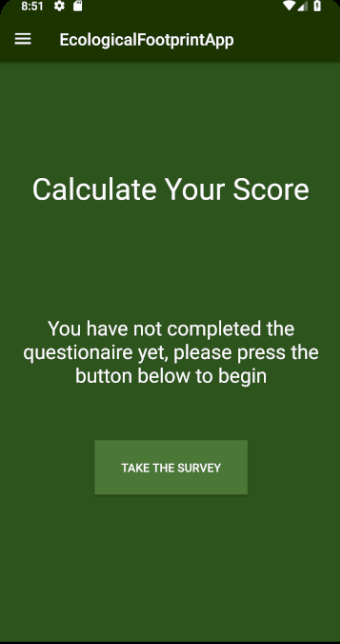
\includegraphics[width=50mm]{Homeiter1.png}
\caption{Current iteration of the home screen. Will prompt users to take the survey if they have not done so before.}
\label{fig:method}
\end{figure}

\begin{figure}[h!]
\centering
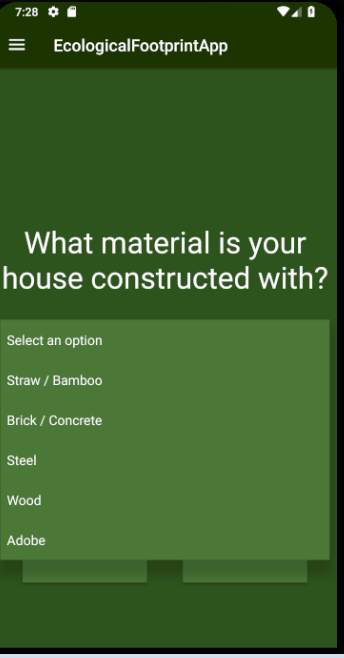
\includegraphics[width=50mm]{QuestionIter1.png}
\caption{Current iteration of a question screen. The text and answers have been updated, this is one of fifteen questions that will be asked.}
\label{fig:method}
\end{figure}

\begin{figure}[h!]
\centering
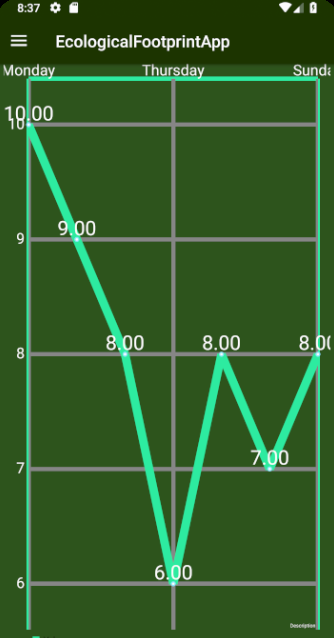
\includegraphics[width=50mm]{TrackingIter1.png}
\caption{Current iteration of the score tracking screen. Uses a line chart to display score change over time.}
\label{fig:method}
\end{figure}

\begin{figure}[h!]
\centering
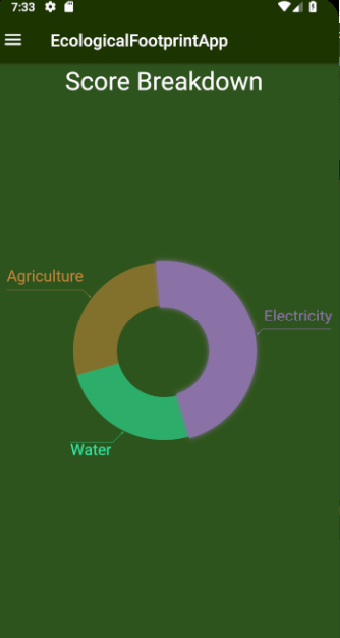
\includegraphics[width=50mm]{BreakdownIter1.png}
\caption{Current iteration of the score breakdown screen. Uses an animated pie chart to display what answers contribute most to a user's score.}
\label{fig:method}
\end{figure}

\begin{figure}[h!]
\centering
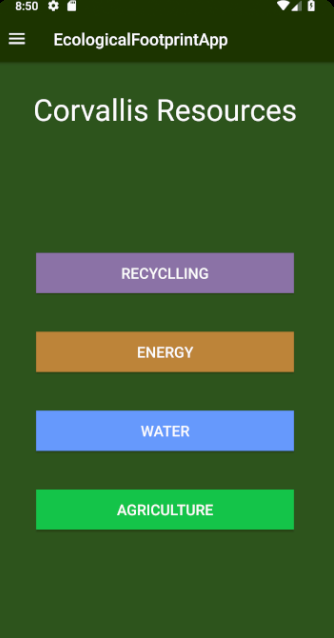
\includegraphics[width=50mm]{CorvallisIter1.png}
\caption{Current iteration of the Corvallis resources screen. This screen will contain resources for Corvallis locals that may help them reduce their score or otherwise learn more about relevant information specific to the Corvallis area.}
\label{fig:method}
\end{figure}

\begin{figure}[h!]
\centering
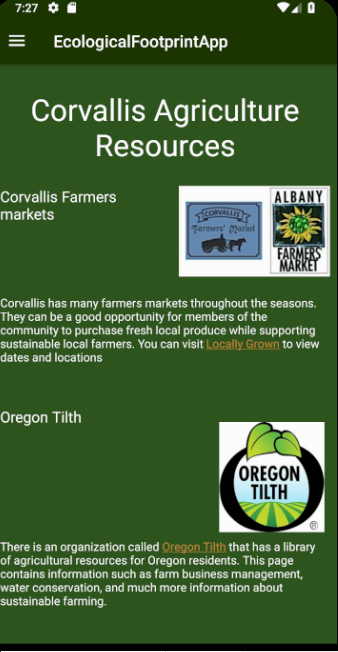
\includegraphics[width=50mm]{AgricultureResources.png}
\caption{Current iteration of the agriculture section of Corvallis Resources. This section is intended to provide local resources for reducing impact.}
\label{fig:method}
\end{figure}




\end{document}